\begin{frame}
	\frametitle{Análise assintótica}
	\framesubtitle{Limites assintóticos - O que é uma assíntota?}
	\begin{columns}
		\begin{column}{0.5\textwidth}
			\par Dada uma $f(x)=b$ uma assíntota é a curva dada pela equação \ref{eq:assintota}.
			\begin{equation}
				\lim_{x\to\infty} f(x) = b \qquad,
				\label{eq:assintota}
			\end{equation}
		\end{column}
		\begin{column}{0.5\textwidth}
			\begin{figure}
				\centering
				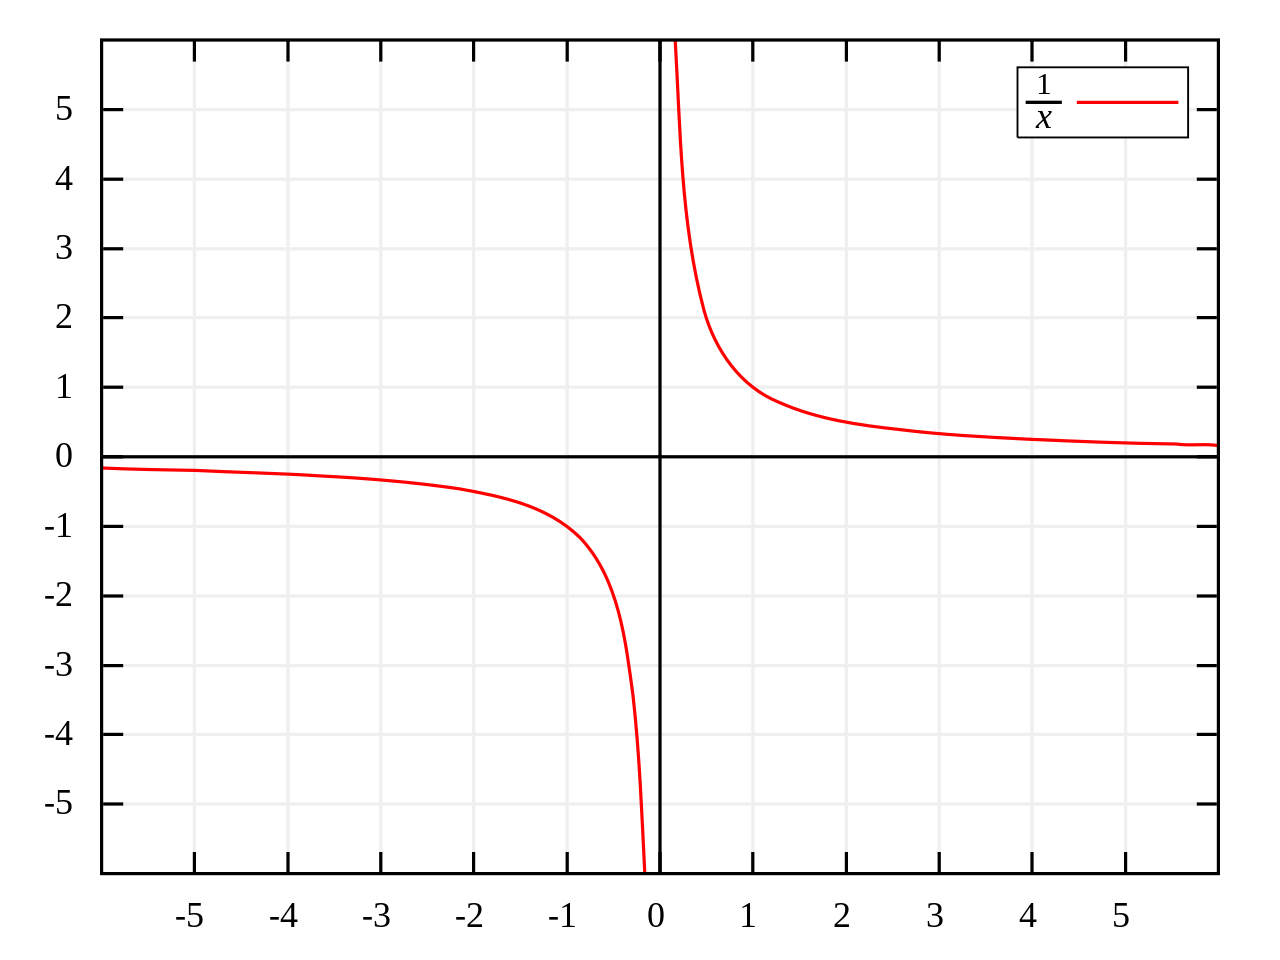
\includegraphics[width=.9\linewidth]{images/assintotas}
				\caption{A função f(x)=1/x tem como assíntotas os eixos coordenados. Fonte: Wikipedia}
				\label{fig:assintotas}
			\end{figure}
		\end{column}
	\end{columns}
\end{frame}

\begin{frame}[fragile]
	\frametitle{Análise assintótica}
	\framesubtitle{Antes começar}
	
	\par Antes de fazer a análise assintótica é necessário aprender a contar o número de instruções primitivas que estão sendo executadas. Geralmente se considera apenas algumas operações elementares como comparações e atribuições.	
\end{frame}

\begin{frame}[fragile]
	\frametitle{Análise assintótica}
	\framesubtitle{Contagem}
	
	\begin{lstlisting}[language=C++, caption={Um algorítimo de tempo constante}, label={lst:umAlgo}]
		
		int valor = 0; 									//Custo 1
		int vetor[] = int[100];					//Custo 1
		for (i=0; i < 100; i++){				// <- 100 vezes
			soma += vetor[i];							//Custo 1
		}
		
		std::cout << soma << std::endl;	//Custo 1
	\end{lstlisting}
	
	
	\begin{lstlisting}[language=C++, caption={Um algorítimo de tempo variável}, label={lst:umAlgo}]
		
		int somatorio(int n, int vetor[]){
			
			int valor = 0; 						//Custo 1
			for (i=0; i < n; i++){		// <- n vezes
				soma += vetor[i];				//Custo 1
			}
			
			return soma;							//Custo 1
		}
	\end{lstlisting}
	
	
\end{frame}

\begin{frame}
	\frametitle{Análise assintótica}
	\framesubtitle{Classes de comportamento assintótico}
	\par Em ordem de tempo crescente:
	\begin{itemize}
		\item $1$ - constante
		\item $\log n$ - logarítimica
		\item $n$ - linear
		\item $n.\log n$ - logarítimica
		\item $n^2$ - quadrática, cúbica, etc. 
		\item $2^n$ - exponencial
		\item $n!$ - fatorial
		\item $n^n$ - vixi...
	\end{itemize}
	\par Ver o exemplo \textit{ordensDeComportamento.ipynb} no jupyter-lab.
\end{frame}

\begin{frame}[fragile]
	\frametitle{Limites assintóticos}
	\framesubtitle{Limites inferiores e superiores}
	\par O limite superior de um algoritmo é o \textbf{maior tempo} que o mesmo leva para executar.
	\par O limite inferior é o \textbf{menor tempo}. 
	\lstinputlisting[language=c++]{codigo/melhorPiorCaso.cpp}
	\par Dependendo do valor do menor elemento o comportamento do algorítimo muda. Testemos o código acima com $vetor = \{1,2,3,4,5\}$ e com $vetor = \{10,5,3,2,-4\}$ e $n = 5$.
\end{frame}

\begin{frame}
	\frametitle{Limites assintóticos}
	\framesubtitle{Limites inferiores e superiores}
	\par \textbf{Melhor Caso}: $1 + 1*n + 1 + 1 + 1 = n + 4$ (linear)
	\par \textbf{Pior Caso}: $1 + 2*n + 1 + 1*n*n + 1 = n2 + 2n + 3$ (quadrático)\newline
	\par A complexidade desse algoritmo pode ser descrita como: $\Omega(n)$ e $O(n^2)$
	\begin{figure}
		\centering
		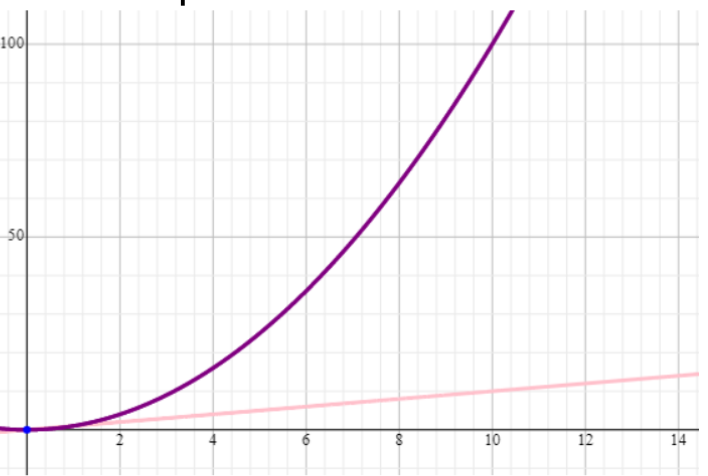
\includegraphics[width=0.4\linewidth]{images/primeiroOmegaOzao}
		\caption{Gráfico do comportamento do algorítimo}
		\label{fig:primeiroomegaozao}
	\end{figure}
	
\end{frame}

\begin{frame}
	\frametitle{Limites assintóticos}
	\framesubtitle{Limites inferiores e superiores - Exercicios}
	\par Como já foi dito o tempo do algoritmo pode variar segundo a entrada de dados, considerando isto, se faz necessário avalia-lo segundo seu \textbf{melhor} e \textbf{pior} caso de execução.
	
	O melhor caso de execução é aquele que no qual o algoritmo leva menos tempo (executa menos comandos) o pior é aquele que ocupa mais.
\end{frame}

\begin{frame}[fragile]
	\frametitle{Limites assintóticos}
	\framesubtitle{Limites inferiores e superiores - Exercícios}
	\begin{lstlisting}[language=C++,caption={Algoritmo 1}]
		int soma = 0;
		for (int i=0; i<n; i++)
		soma = soma + i;
	\end{lstlisting}
	
	\begin{lstlisting}[language=C++,caption={Algoritmo 2}]
		int soma1 = 0;
		int soma2 = 0;
		for (int i=0; i<n; i++){
			soma1 = soma1 + 1;
			soma2 = soma2 + i;
		}
	\end{lstlisting}
	
\end{frame}

\begin{frame}[fragile]
	\frametitle{Limites assintóticos}
	\framesubtitle{Limites inferiores e superiores - Exercícios}
	
	\begin{lstlisting}[language=C++,caption={Algoritmo 3}]
		int soma1 = 0;
		for (int i=0; i<n; i++){
			soma1 = soma1 + 1;
		}
		for (int j=0; j<n;j++){
			soma1 = soma1 + j;
		}
	\end{lstlisting}
	
	\begin{lstlisting}[language=C++,caption={Algoritmo 4}]
		int soma = 0;
		for (int i=0; i<n; i++){
			for (int j=0; j<m; j++){
				soma = soma + 1;
			}
		}
	\end{lstlisting}
	
\end{frame}

\begin{frame}[fragile]
	\frametitle{Limites assintóticos}
	\framesubtitle{Limites inferiores e superiores - Exercícios}
	
	\begin{lstlisting}[language=C++,caption={Algoritmo 5}]
		int menor = INT_MAX;
		for (int i=0; i<n; i++){
			if (vetor[i] < menor)
			menor = vetor[i];
		}
	\end{lstlisting}
	
\end{frame}

\begin{frame}
	\frametitle{Análise assintótica}
	\framesubtitle{Limites}
	\par Atribui limites superiores, exatos e inferiores para o tempo de execução de um algorítimo expressando os mesmos em forma de funções assintóticas a esse tempo de execução.\newline
	\par Para fazer essa análise usaremos código real e/ou pseudo-código: \textbf{Cuidado com as chamadas informais}.\newline
	
	\par Se assume que o acesso a RAM e as operações primitivas na CPU também tenham um tempo constante.
	\begin{itemize}
		\item o - Limite assintótico superior de ordem superior.
		\item O - Limite assintótico superior.
		\item $\theta$ - Limite assintótico restrito.
		\item $\Omega$ - Limite assintótico inferior.
		\item $\omega$ - Limite assintótico inferior de ordem inferior.
	\end{itemize}
\end{frame}

\begin{frame}
	\frametitle{Limites assintóticos}
	\framesubtitle{Relações entre os comportamentos assintóticos}
	\par Se um algorítimo \textbf{não} é $O$ então também não será $o$
	\par Se o algorítimo é $O$ e $\Omega$ o mesmo não será $\Theta$.
	\par Se o algorítimo é $\Theta$ então não poderá ser $\omega$ ou $o$.
	\par Se o algorítimo é $O$ e \textbf{não} é $\Omega$ então não poderá ser $\Theta$.
	\par Se é $o$ ou $\omega$ então \textbf{não} é $\Theta$. 
\end{frame}

\begin{frame}
	\frametitle{Limites assintóticos}
	\only<1>{
		\framesubtitle{Mas... espera um pouco...}
		\begin{columns}
		\begin{column}{0.8\textwidth}
			\begin{figure}
				\centering
				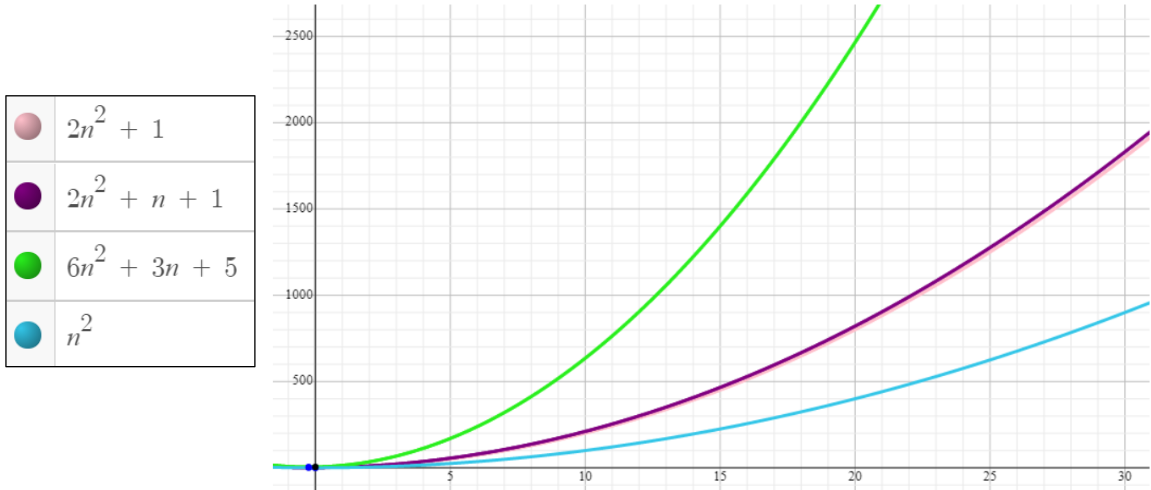
\includegraphics[width=\linewidth]{images/assintotas2}
				\caption{Assíntotas de $n^2$}
				\label{fig:assintotas2}
			\end{figure}
		\end{column}
		\begin{column}{0.2\textwidth}
			\par Como pode $O(n^2)$ ser o limite assintótico superior se $n^2 \le 6n^2+3n+5$ ?
		\end{column}
		\end{columns}
	}
	\only<2>{
		\framesubtitle{Notação "Ózão" (ou \textit{big O})}
		\par Na notação "Ózão" (ou \textit{big O}) se diz que uma função $f(x)$ domina assintoticamente uma função $g(n)$ quando existem constantes $c$ e $a$ tais que, para \textbf{qualquer} $n \geq a$ é verdadeiro que $c.f(n) \geq g(n)$.\newline
		\par De outra forma podemos dizer que:\newline
		
		\begin{itemize}
			\item $g(n) = O(f(n))$
			\item $g(n)$ é da ordem no máximo $f(n)$
			\item $g(n)$ é $O$ de $f(n)$
			\item $g(n)$ é igual a $O$ de $f(n)$
			\item $g(n)$ pertence a $O$ de $f(n)$
		\end{itemize}
		
		\par Ver o exemplo \textit{ordensDeComportamento.ipynb} no jupyter-lab.
	}
\end{frame}